% Format teze zasnovan je na paketu memoir
% http://tug.ctan.org/macros/latex/contrib/memoir/memman.pdf ili
% http://texdoc.net/texmf-dist/doc/latex/memoir/memman.pdf
% 
% Prilikom zadavanja klase memoir, navedenim opcijama se podešava 
% veličina slova (12pt) i jednostrano štampanje (oneside).
% Ove parametre možete menjati samo ako pravite nezvanične verzije
% mastera za privatnu upotrebu (na primer, u b5 varijanti ima smisla 
% smanjiti 
\documentclass[12pt,oneside]{memoir} 




% Paket koji definiše sve specifičnosti master rada Matematičkog fakulteta
\usepackage[latinica]{matfmaster} 
%
% Podrazumevano pismo je ćirilica.
%   Ako koristite pdflatex, a ne xetex, sav latinički tekst na srpskom jeziku
%   treba biti okružen sa \lat{...} ili \begin{latinica}...\end{latinica}.
%
% Opicija [latinica]:
%   ako želite da pišete latiniciom, dodajte opciju "latinica" tj.
%   prethodni paket uključite pomoću: \usepackage[latinica]{matfmaster}.
%   Ako koristite pdflatex, a ne xetex, sav ćirilički tekst treba biti
%   okružen sa \cir{...} ili \begin{cirilica}...\end{cirilica}.
%
% Opcija [biblatex]:
%   ako želite da koristite reference na više jezika i umesto paketa
%   bibtex da koristite BibLaTeX/Biber, dodajte opciju "biblatex" tj.
%   prethodni paket uključite pomoću: \usepackage[biblatex]{matfmaster}
%
% Opcija [b5paper]:
%   ako želite da napravite verziju teze u manjem (b5) formatu, navedite
%   opciju "b5paper", tj. prethodni paket uključite pomoću: 
%   \usepackage[b5paper]{matfmaster}. Tada ima smisla razmisliti o promeni
%   veličine slova (izmenom opcije 12pt na 11pt u \documentclass{memoir}).
%
% Naravno, opcije je moguće kombinovati.
% Npr. \usepackage[b5paper,biblatex]{matfmaster}







% Datoteka sa literaturom u BibTex tj. BibLaTeX/Biber formatu
\bib{marina-master}

% Ime kandidata na srpskom jeziku (u odabranom pismu)
\autor{Marina R. Nikolić}
% Naslov teze na srpskom jeziku (u odabranom pismu)
\naslov{Prikupljanje i prikaz podataka o izvršavanju programa}
% Godina u kojoj je teza predana komisiji
\godina{2018}
% Ime i afilijacija mentora (u odabranom pismu)
\mentor{dr Milena \textsc{Vujošević Janičić}, docent\\ Univerzitet u Beogradu, Matematički fakultet}
% Ime i afilijacija prvog člana komisije (u odabranom pismu)
\komisijaA{dr Filip \textsc{Marić}, vanredni profesor\\ Univerzitet u Beogradu, Matematički fakultet}
% Ime i afilijacija drugog člana komisije (u odabranom pismu)
\komisijaB{dr Milan \textsc{Banković}, docent\\ Univerzitet u Beogradu, Matematički fakultet}
% Ime i afilijacija trećeg člana komisije (opciono)
% \komisijaC{}
% Ime i afilijacija četvrtog člana komisije (opciono)
% \komisijaD{}
% Datum odbrane (odkomentarisati narednu liniju i upisati datum odbrane ako je poznat)
% \datumodbrane{}

% Apstrakt na srpskom jeziku (u odabranom pismu)
\apstr{tekst apstrakta rada
}

% Ključne reči na srpskom jeziku (u odabranom pismu)
\kljucnereci{profajliranje, pokrivenost koda, GCC, GCOV}

\begin{document}
% ==============================================================================
% Uvodni deo teze
\frontmatter
% ==============================================================================
% Naslovna strana
\naslovna
% Strana sa podacima o mentoru i članovima komisije
\komisija
% Strana sa posvetom (u odabranom pismu)
\posveta{Mentoru za predanost i pomoć, firmi za resurse, porodici i prijateljima za podršku}
% Strana sa podacima o disertaciji na srpskom jeziku
\apstrakt
% Sadržaj teze
\tableofcontents

% ==============================================================================
% Glavni deo teze
\mainmatter
% ==============================================================================

% ------------------------------------------------------------------------------
\chapter{Uvod}
% ------------------------------------------------------------------------------


\begin{enumerate}
\item kratak opis o čemu će biti reči u daljem tekstu
\item iako vidim da je popularno po master radovim ada se piše po poglavljima ovde (tipa, u poglavlju X je opisano to i to), ja bih uvod radije sročila kao pričicu koja prati rad
\item ovde bih dodala na samom početku i na samom kraju značaj teme kao takve i naravno značaj mog doprinosa ( na kraju zbog efekta)
\end{enumerate}


% ------------------------------------------------------------------------------
\chapter{Profajliranje, pokrivenost koda i kako sad radi GCC}
\label{chp:profajliranje}
% ------------------------------------------------------------------------------

\section{Profajliranje i pokrivenost koda}


\subsection{Uvod}

Razvoj softvera je znatno širi pojam od pisanja koda. Obuhvata više, podjednako važnih segmenata, kao što su: planiranje, analiza i usklađivanje sa zahtevima klijenata, testiranje, analiza performansi, optimizacija, održavanje i mnogi drugi. Samo investiranjem u svaki ponaosob, može se proizvesti kvalitetan i dugotrajan softver. Njihova kompleksnost proporcijano raste sa značajem i složenošću krajnjeg proizvoda, iz čega proističe i važnost njihovog olakšavanja. Postoje brojne metodologije i tehnike koje su specijalizovane za vođenje procesa karakterističnih za rane faze razvoja, kao što su planiranja ili analize zahteva. Međutim, ovaj rad će se usresrediti na prikaz onih koje olakšavaju procese kasnog razvoja, pre svega testiranja i optimizacije. Za uspešno sprovođenje tih procesa, važan faktor je odabir tehnika koje će se primenjivati i jedinica koda kome su oni najneophodniji, a kvalitetan odabir je uslovljen dobrim poznavanjem samog softvera, njegovih karakteristika i ponašanja. Takvu vrstu informacije obezbeđuje analiza programa.

\subsection{Analiza programa}

Analiza programa predstavlja automatizovani proces analiziranja raznih aspekata softvera, pre svega njegovog ponašanja, u različitim slučajevima upotrebe, u cilju olakšavanja procesa testiranja korektnosti, naročito eksterno nabavljenih delova softvera, procene performansi i optimizacije. Pruža korisne informacije o raspodeli potrošnje resursa, čvorovima ekstremne potrošnje, potencijalnim kritičnim segmentima izvršavanja, korektnosti toka izvršavanja i slično. Poput projekta veštačke inteligencije, njen krajnji cilj je stvaranje "pametnog prevodioca", koji bi mogao automatski generisati efikasan, a pouzdan kod. Značaj njenih trenutnih mogućnosti, kao i brzina kojom se unapređuje, ukazuju na veliku verovatnoću ostvarljivosti tog cilja. Analiza programa je veoma širok pojam, koji obuhvata veliki broj vrlo raznovrsnih metoda, ali se može veoma precizno podeliti na dva osnovna tipa. To su statička i dinamička analiza.

\subsection{Statička analiza programa}

Statička analiza programa \cite{Static} obuhvata sve metode i tehnike utvrđivanja ponašanja programa, za koje ga nije potrebno izvršiti. Sve procedure se vrše nad izvornim kodom i, prikupljajući podatke o njegovoj strukturi, generišu korisne informacije o mogućim ishodima njegovog budućeg izvršavanja. Primer su mnogobrojne softverske metrike, koje na osnovu podataka o broju linija, klasa ili metoda, izračunavaju takozvani "statistički kvalitet" softvera. 

Njena glavna prednost proističe upravo iz toga, što kod nije potrebno izvršiti. Ovakvim ograničenjem se često odlikuje razvoj velikih i skupih softverskih sistema, gde se zbog materijalnih mogućnosti ne može vršiti testiranje svih manjih jedinica u realnom okruženju. Kao ilustrativan primer se može posmatrati razvoj softera za automatsko navođenje rakete i jedan manji segment tog razvoja koji predstavlja program za izračunavanje potrošnje goriva prilikom jednje vožnje. Testiranje korektnosti sastavne jedinice te veličine se u najvećoj meri vrši na simulatorima. Lansiranje prave rakete za potrebe ovakvog testiranja je ekonomski neopravdano, iako okruženje koje simulator pruža ne obuhvata sve alternativne slučajeve upotrebe. 

Sa druge strane, ukoliko uzmemo u obzir činjenicu da vreme izvršavanja proizvoljnog programa može biti proizvoljno dugo, iz neneophodnosti izvršavanja, može se izvesti još jedna velika prednost statičke analize, a to je brzina. Faktor brzine čini osnovu ocene svakog pristupa.

Iz nenophpodnosti izvršavanja, proističe još jedna velika prednost statičke analize, a to je nepsristrasnost. Nezavisnost od ulaznih podataka i okruženja, omogućava efikasnu detekciju graničnih slučajeva.
 
Osnovne mane statičke analize su uzrokovane uskom vezom njenih tehnika sa statistikom kao naukom i predstavljaju nepreciznost i smanjenu informativnost o praktičnim slučajevima upotrebe. Njeni rezultati nisu eksperimentalne prirode, već prikazuju teorijsko predviđanje ponašanja. Zbog toga se ne trebaju smatrati potvrdama ispravnosti ili performansi, već isključivo tretirati kao smernice pri razvoju.

\subsection{Dinamička analiza programa}

Dinamička analiza programa \cite{Gupta} obuhvata sve metode i tehnike prikupljanja podataka o programu tokom njegovog izvršavanja i utvrđivanja ponašanja programa na osnovu tih podataka. Procedure uglavnom započinju u fazi prevođenja, ali najvažniji deo se obavlja u toku i nakon izvršavanja. Pored strukture koda i statičkih podataka, na njen ishod utiču i ulazne vrednosti, kao i parametri okruženja. Testovi jedinica koda, sistemski testovi i testovi prihvatljivosti koriste isključivo ovaj vid analize programa. 

Sve njene glavne prednosti u odnosu na statičku analizu, proističu iz uticaja "realnih parametara". Određene mane softverskih rešenja ispoljavaju se samo u toku rada tog softvera, a mnoge i proističu upravo iz spoljnih faktora ili veze sa njima. Statistički savršen softver koji je nedovoljno primenljiv u praksi, predstavlja jedan od tri osnovna neuspeha prilikom razvoja softvera \cite{Malkov}. Marketinška istraživanja, analize zahteva korisnika i detaljni popisi slučajeva upotrebe se primenjuju u ranim fazama softvera u cilju zaštite od ove vrste neuspeha. Međutim, pojedini faktori okruženja, poput vrednosti jedne jedinice iz skupa obrade, tzv. "lažne pozitivne ili negativne vrednosti", se ne mogu detektovati metodama koje se baziraju na statistici. Posledice obuhvataju brojna prilagođavanja i održavanja u kasnim fazama razvoja, koja se neretko završavaju odustajanjem od razvoja nakon isteka novčanih sredstava ili pronalaska kvalitetnijeg rešenja. Zbog toga su testiranja u realnom okruženju veoma važna, a kako su po svojoj prirodi ograničena resursima, važno je i iz njih ekstrahovati što više informacija za naredne iteracije razvoja. Njih obezbeđuje dinamička analiza programa.

 
Važna prednost dinamičke analize je i univerzalnost, koja proističe iz činjenice da se sve tehnike primenjuju na izvršnu verziju, bez neophodnog prisustva izvornog koda. Oblast primene je šira, jer obuhvata i programe sa "zatvorenim" kodom. Pisanje celokupnog koda softvera je skupo, kako u ekonomskom, tako i u pogledu utrošenog vremena, zbog čega ne predstavlja dovoljno kompetetivan način proizvodnje. Ovaj princip nije karakteristika samo softverske industrije, već je globalna odlika industije kao grane privrede. Kao ilustrativan primer se može posmatrati javni prevoz građana i porediti cena jedne autobuske karte u odnosu na cenu goriva i održavanja automobila, na relaciji od nekoliko kilometara. Ukupna cena jednog prevoza se ravnomerno raspoređuje na više putnika, čime je pojedinačna cena po putniku znatno manja. Sa druge strane, prevoznik nema obavezu da proizvod ustupi za tačnu cenu pojedinačnog dela, iz čega proističe njegova zarada. Cena održavanja automobila je dodata u ilustraciju, u cilju naglašavanja troškova održavanja softvera, koje često predstavlja najveći materijalni ishodak razvoja.U razvoju softvera, ovaj princip se ogleda u eksternom nabavljanju komponenti, u kom slučaju se često može kupiti samo izvršna verzija. Izvorni kod predstavlja poslovnu tajnu proizvođača. Procene kvaliteta pre integracije, kao i testiranje kompatibilnosti sa ostatkom softvera, stoga se mogu obaviti jedino dinamičkim pristupom. 

Najveća mana ovog pristupa jeste potencijalni osećaj lažne sigurnosti. To je, u određenoj meri, neizostavna stavka svakog testiranja. Neiskusni razvojni timovi se mogu previše osloniti na rezultate analize i time prevideti činjenicu da ona, kao automatizovani proces, ne može garantovati stoprocentnu tačnost. Alati koji je vrše su takođe softverski proizvodi, i samim tim jednako podložni greškama koliko i kod koji se njima analizira. Posebno mesto u tehnikama dinamičke analize ima profajliranje, i njemu će ovaj rad biti u potpunosti posvećen. 

\subsection{Profajliranje}

Profajliranje \cite{PGO} \cite{Verifikacija} predstavlja prikupljanje raznih podataka iz izvršavanja programa u realnom ili simuliranom okruženju, koji pružaju uvid u tok i performanse rada programa. Obradom ovih podataka, dobijaju se vredne informacije o vremenskim i memorijskim zahtevima programa, složenosti i iskorišćenosti pojedinih delova koda i slično. Rezultati rada alata za profajliranje predstavljaju korisne smernice za procese testiranja i optimizacije, jer ukazuju na delove koda kojima su oni najneophodniji.


Ulazne vrednosti i parametri okruženja, zajedno sa kodom programa, jedinstveno određuju tok izvršavanja. Uočavanje pozitivnih podataka o izvršavanju van predviđenog toka, ili negativnih u njegovoj unutrašnjosti, za unapred određen slučaj upotrebe, je stoga dobar pokazatelj da se u kodu nalaze greške. Štaviše, pruža i dodatnu olakšicu za budući proces "debagovanja", sužavanjem oblasti pretrage. Detekcija memorijski ili vremenski izrazito zahtevnih segmenata, kao i segmenata koji se veoma često izvršavaju usmerava pažnju razvojnog tima na neophodnost optimizacije, pritom takođe obezbeđujući dodatnu informaciju gde je ona i koliko potrebna. Poređenjem performansi različitih verzija koda, može se izvršiti dobra procena kvaliteta i odabir odgovarajućeg algoritma u ranim fazama, kada je njegova zamena u velikoj meri jeftinija. Smernice koje profajleri daju mogu znatno "očistiti" kod od nepotrebnih grananja, invarijanti petlji pogrešno smeštenih unutar same petlje, "mrtvog koda" i sličnih propusta. Stoga značajno olakšavaju i proces refaktorisanja koda. Vrši se alatom koji se naziva profajler i sastoji se od tri usko spregnute faze: instrumentalizacija, prikupljanje i obrada podataka.

\subsection{Faze profajliranja. Instrumentalizacija}

Instrumentalizacija \cite{SCI} koda predstavlja sposobnost merenja karakteristika programa, koja se postiže ubacivanjem dodatnih instrukcija u program tokom prevođenja. Instrukcije predstavlju kod inicijalizacija određenih dodatnih struktura za instrumentalizaciju i pravila za njihovo popunjavanje. Dodatne strukture imaju ulogu skladišta za metapodatke, a za popunjavanje je zadužen sam instrumentalizovani program. Time se stvara opterećenje i smanjuju performanse, ali je, iz više razloga, najpouzdanije i najoptimalnije moguće rešenje. Prvenstveno, iz ugla bezbednosti. Neograničen pristup internim podacima jednog programa ne sme imati niko sem njega samog. Time bi se otvorile brojne mogućnosti za razvoj novog malicioznog softvera koji bi zloupotrebio ovaj bezbednosni propust, bilo napadajući alat za instrumentalizaciju, bilo poruke koje razmenjuje sa instrumentalizovanim programom. Zaštita u vidu šifrovanja bi zahtevala dodatno trošenje resursa, što nije isplativo. Pored bezbednosnog aspekta, bitan faktor je i sinhronizacija. U sistemu sa eksternim alatom, usklađivanje čitanja i pisanja memorijskih segmenata dodeljenih programu bi iziskivalo dodatno trošenje procesorskog vremena i memorije, a i zaključavanje bi povećalo vremensku složenost.

Faza prikupljanja podataka obuhvata: čitanje dodatnih struktura sa metapodacima, njihovo konvertovanje u pogodniji oblik i eksterno skladištenje. Da bi oblik bio pogodan, neophodno je da predstavlja dobar balans između veličine, koja treba biti što manja, i informativnosti, koja treba biti što veća. Ukoliko neki podaci mogu da se izvedu iz ostalih, oni se eliminišu. Lokacija podataka u eksternom skladištu predstavlja memorijski besplatan podatak, koji omogućava dodatnu kompresiju bez gubitka na informativnosti. Ova faza je takođe poverena samom programu, iz istih razloga kao i instrumentalizacija.

Produkt prve dve faze su sirovi podaci, koji u sebi nose informacije o karakteristikama programa u realnim slučajevima upotrebe, ali kako se podaci prikupljaju samo ako program ima dodatnu funkciju da u toku rada prikuplja i svoje metapodatke, ne može se obezbediti potpuna preciznost informacija. Uticaj se ne može u potpunosti ukloniti, međutim mora biti sveden na granicu prihvatljivosti. Ispravna instrumentalizacija ne sme uticati na funkcionalnost programa, ni algoritamski, ni umanjenjem performansi. 

Poslednja faza predstavlja obradu sirovih podataka do korisne informacije. Krajnji proizvod predstavlja jedan ili više izveštaja u formatu pogodnom prvenstveno za razvojni tim, ne za računar. Osnovne karakteristike izveštaja treba da budu: uniformnost, preglednost, povišena (vraćanje izvedenih podataka) ili snižena informativnost (filtriranje podataka po kategorijama), unija pojedinačnih i statističkih prikaza i slično. Ovu fazu obično obavljaju eksterni alati, jer je potpuno nezavisna od izvršavanja programa i njegove interne memorije. U zavisnosti od toga koje se karakteristike mere i potreba korisnika, krajnji izveštaji variraju od jednorečeničnih ispisa, preko kolekcija fajlova, do interaktivnih aplikacija. Mogu se meriti razne karakteristike, poput na primer memorijskih zahteva ili tragova izvršavanja, ali se po informativnosti i univerzalnosti primene ističe se pokrivenost koda.

\subsection{Pokrivenost koda}

Pokrivenost koda \cite{Introduction} \cite{Testing} \cite{Ecl} \cite{Warrning} \cite{Misuse} \cite{Pizza} predstavlja "stepen izvršenosti koda". Izračunava se kao odnos broja izvršenih i neizvršenih linija, blokova, grana ili funkcija i izražava se u procentima. U strogom smislu, pokrivenost koda je jedan jedini broj, dobijen merenjem nad celim sistemom. Taj broj je sam po sebi veoma informativan. Što je pokrivenost manja, to je verovatnoća da u kodu postoje ozbiljne greške u logici veća. 

Međutim, nakon merenja na celom skupu, poželjno je izvršiti i merenja na manjim segmentima: komponentama, klasama ili funkcijama, kako bi se detektovali propusti globalne informacije. Na primer, ukoliko je stil pisanja koda takav da se po fajlovima grupišu slični metodi iz različitih klasa, ovakvim pristupom mogu se bolje detektovati slabo ili nimalo korišćene klase, ili objekti koji se prave i uništavaju bez da utiču na ukupnu funkcionalnost. Podaci o izvršavanju konkretnih linija, mogu doprineti pronalasku invarijanti petlje slučajno smeštenih u njenu unutrašnjost ili bespotrebnih grananja koja se svedu na isti krajnji rezultat. Stoga, pokrivenost koda ne treba shvatati samo u svom najužem smislu, već maksimalno iskoristiti sve njene mogućnosti. Uzroci neočekivane pokrivenosti mogu biti veoma raznovrsni. U daljem tekstu biće predstavljeno nekoliko primera. 

Stariji softveri koji se duže vreme održavaju, neretko sadrže visok procenat koda iz prethodnih verzija, koji je vremenom izgubio svoju funkcionalnost. Smenom razvojnih timova, naročito u okruženjima koja ne podržavaju detaljno dokumentovanje učinka, često se gube informacije o funkcionalnosti pojedinih delova koda. Usled nedostatka informacija, novi razvijaoci se često ne odlučuju na eliminisanje ili zamenjivanje delova koda, već se uglavnom vrši dodavanje. Funkcije ili klase, a neretko i čitave komponente, tako postaju "mrtav kod", koji otežava procese održavanja i "debagovanja". Ovakvi softveri imaju naročito malu pokrivenost.

Važan faktor prilikom razvoja softvera predstavlja i balans između preciznosti i brzine. Preopterećivanje programa ispitivanjem malo verovatnih alternativnih slučajeva, dovodi do slabljenja performansi. Pored toga, suvišna grananja mogu proizvesti ogromne količine mrtvog koda, od linija pa do čitavih klasa ili komponenti pisanih isključivo za te specijalne slučajeve. To znatno otežava održavanje koda, debagovanje i refaktorisanje. Mala pokrivenost može biti dobar pokazatelj, a podaci izvršavanja linija odrediti preciznije lokaciju problema.

Gotovo sve današnje sisteme odlikuje konkurentno ili paralelno izvršavanje. Njima se postiže značajan porast efikasnosti, ali i povećava broj potencijalnih problema koji mogu nastati prilikom izvršavanja, poput živih i mrtvih zaključavanja, ili trke za resurse. Ovi problem mogu uzrokovati blokiranje ili prestanak rada celog sistema, a njihovo blagovremeno otkrivanje je gotovo nemoguće. Algoritam rada procesora određuje koji će se proces, kada i koliko izvršavati, a programer može jedino implementirati neke vidove zaštite atomičnosti operacija ili nametanja prioriteta procesa. Međutim, i pored zaštitnih mehanizama, dešava se da se nekim procesima ne dodeli vreme na procesoru. Takvi kodovi imaju izuzetno niske pokrivenosti, a najbolji pokazatelj su pokrivenosti pojedinačnih izvršavanja koje iznose nula procenata. Prilikom rada sa nitima, niske pokrivenosti mogu biti simptom i preopterećenosti. 

Najozbiljniji problemi koji uzrokuju malu pokrivenost su "greške u logici". One mogu varirati, od pogrešno definisanih uslova u granama ili petljama do potpuno promašenih algoritama. Neočekivana generalna pokrivenost je dobar pokazatelj da u kodu ima ovakvih grešaka. Pokrivenost manja od očekivane može, na primer, biti uzrokovana pozivom pogrešnih funkcija, ulaskom u neproduktivnu granu ili prevremenim izlaskom iz programa. Veća pokrivenost od očekivane može biti simptom nepravilnog rada uslova u naredbi grananja, loše konstruisanih provera u kodu i slično. Kako uzroci mogu biti veoma raznovrsni, dobro je pored generalne, meriti i pokrivenosti na segmentima. Kombinovanjem svih rezultata, sužava se oblast pretrage i lako locira greška u logici. 

Jedina potvrda ispravnosti koda pre nego što ode u produkciju su dobri rezultati testiranja. Međutim, na ishod testova ne utiču samo karakteristike softvera koji se testira, već i njihova ispravnost. Testovi se često sami ne testiraju dovoljno dobro, što može dovesti do ozbiljnih posledica. Lažan negativan rezultat može uzrokovati bespotrebnu potrošnju vremena i novca na traženje nepostojeće greške u kodu. Lažan pozitivan rezultat može imati još i ozbiljnije posledice, čija težina zavisi od važnosti samog softvera. Stoga je veoma korisno primeniti tehniku određivanja pokrivenosti koda i na testove, a ne samo na primarni softver. Mala pokrivenost je dobar indikator da u kodu postoje segmenti koji nisu testirani, a koji su samim tim potencijalna opasnost. 

Računanjem pojedinačnih pokrivenosti možemo doći i do informacija o često korišćenim segmentima koda. One umnogome olakšavaju razvojnom timu prilikom donošenja odluka vezanih za vremensku optimizaciju. Kombinovanjem sa podacima za pojedinačne linije koje alociraju memoriju, mogu se pronaći memorijski zahtevni segmenti koji su dobri kandidati za prostornu optimizaciju.

Najsitniji podaci, poput podataka o izvršavanju pojedinih linija ili blokova se mogu koristiti i za refaktorisanje. Uklanjanjanje mrtvog koda ili razbijanje preopterećenih funkcija, su samo neki od primera refaktorišućih procesa koji su olakšani uz informacije o pokrivenosti koda, a čije sprovođenje umnogome pospešuje održavanje ili dalji razvoj.

Raznovrsnost gore navedenih primera dokazuje veliki značaj i potencijal pokrivenosti koda. Stoga će, na nju biti u poptunosti skoncentrisan ostatak ovog rada. 

Poznatiji prevodioci, poput GCC-a, ICC-a i Clang-a uglavnom u određenoj meri poseduju ugrađenu podršku za testiranje pokrivenosti koda. Projekat LLVM trenutno prednjači u raznovrsnosti, jer obuhvata i statički i dinamički pristup, uključujući i testiranje u toku izvršavanja. Sa druge strane, GCC trenutno podržava samo statičko testiranje pokrivenosti nakon izvršavanja programa, ali ga odlikuju znatno bolje performanse, pre svega u pogledu memorijske zahtevnosti. Prikupljanje i obrada podataka o pokrivenosti koda u toku izvršavanja programa korišćenjem tehnika GCC-a, kombinuje dobru ideju projekta LLVM i dobre tehnike prevodioca GCC, čime prednjači i u oblasti mogućnosti i u oblasti performansi. U okviru projekta na kome je utemeljen ovaj rad, izvršena je detaljna analiza postojećih mogućnosti u okviru prevodioca GCC i implementirana je podrška za prikupljanje podataka u toku izvršavanja, kao i novi, unapređeni alat za njihov vizuelni prikaz.


\section{Postojeća rešenja u okviru GCCa}


Programski prevodilac GCC sadrži ugrađenu podršku za testiranje pokrivenosti koda, integrisanu u statičku biblioteku za prikupljanje podataka po imenu libgcov i alat za vizuelni prikaz podataka GCOV \cite{GCOV} \cite{CodeCoverage}.

Metapodaci izvršavanja čuvaju se u deljenoj memoriji programa, u listi posebnih, globalno definisanih struktura tipa gcov\_info, čija se inicijalizacija ugrađuje u binarni kod prevođenjem sa posebnim flegovima za instrumentalizaciju: -fprofile-arcs -ftest-coverage. Flegovi se navode tokom prevođenja izvornog koda do objektnog fajla, a simboli koji se njima unose razrešavaju se kasnije u fazi linkovanja.  

Pored insercije instrukcija u binarni kod programa, flegovi za instrumentalizaciju obavljaju još jednu važnu aktivnost, a to je kreiranje dodatnog fajla, odmah pored njemu odgovarajućeg fajla izvornog koda, sa ekstenzijom gcno. To je relativno mali, binarni fajl, koji sadrži sve neophodne statičke informacije o strukturi izvornog koda čijim prevođenjem nastaje. Njegova glavna uloga jeste da predstavlja struktuni kostur budućeg finalnog proizvoda alata, koji će se kasnije nadograditi podacima dobijenim dinamički u toku izvršavanja. Format gcno fajla je utvrđen zajedničkim standardom GCC-a i alata GCOV, koji je specijalizovan i za njegovo tumačenje. Veoma je nečitljiv ljudskom oku, što je uzrokovano maksimalnim stepenom kompresije podataka. Korišćenje specijalnih oznaka, korišćenje pozicije kao interpretacije podatka, kao i pažljivo odabrani minimalni skup potrebnih informacija o strukturi, samo su neke od tehnika kompresije korišćenih u cilju maksimalne štednje memorije. Posebno je važno napomenuti da je čuvanje podataka o strukturi u vidu eksternih binarnih fajlova osnovni uzrok boljih memorijskih performansi GCC instrumentalizacije u odnosu na Clang-ovo profajliranje, pomenute na kraju prethodnog poglavlja, jer garantuje bezbednost od eksplozije veličine samog programa. Dovoljno uvećanje izvršnog fajla može dosvesti do nepravilnosti u radu, a kako memorijski zahtevniji instrumentlizovani program se ponaša drugačije od regularnog, rezultati testiranja neće odražavati realno stanje. Naročito, na sistemima sa veoma ograničenim memorijskim prostorom, GCC instrumentalizacija je jedina moguća.

Svaka struktura tipa gcov\_info iz liste, odgovara tačno jednom instrumentalizovanom objektnom fajlu koji učestvuje u izgradnji programa. Pored osnovnih podataka poput imena fajla ili verzije alata, svaka struktura tipa gcov\_info sadrži i pokazivač na niz struktura tipa gcov\_fn\_info, u kojima se skladišti po nekoliko posebnih brojača za svaku funkciju tog fajla. Na osnovu vrednosti u njima, može se konstruisati podatak o količini izvršavanja bilo koje jedinice koda u okviru te funkcije. Tokom rada programa, vrednosti u brojačima se konstantno ažuriraju, i u svakom trenutku odražavaju realno stanje izvršavanja. Ti podaci predstavljaju jezgro informacije o pokrivenosti koda, ali njih eksterni alat poput GCOV-a ne može direktno koristiti iz više razloga. Prvi razlog je bezbednosne prirode, i velikom merom je obrazložen u prethodnom poglavlju. Eksternim alatima se ni u kom slučaju ne treba obezbediti čitanje internih podataka programa. Detaljno je obrazloženo i pitanje sinhronizacije pisanja i čitanja, koje važi i u ovom slučaju. Naposletku, ovim pristupom bi podaci imali poreklo samo iz jednog izvršavanja, što bespotrebno ograničava mogućnosti alata. 

Rešenje koje je trenutno implementirano u GCC, upravo iz tih razloga, sadrži jednog "posrednika" između instrumentalizovanog programa i eksternih alata, a to je libgcov. Biblioteka, po svojoj prirodi, se ugrađuje u program i time postaje deo njega, što joj daje ekskluzivno pravo pristupa njegovoj deljenoj memoriji. Njen osnovni zadatak je ekstrakcija podataka iz strukture gcov\_info i njihovo konvertovanje u oblik pogodan za obradu eksternim alatom. Statička funkcija gcov\_at\_exit preuzima vrednosti brojača, računa sumarne i statističke podatke i sve zajedno upisuje u posebni binarni fajl sa ekstenzijom gcda u unapred utvrđenom formatu i na unapred utvrđenoj lokaciji. Format gcda fajla je takođe veoma nečitljiv, usled primene sličnih tehnika za kompresiju, kao u slučaju gcno fajla. Generiše se uvek pored objetktnog fajla kome odgovara, u slučaju da fajl sa istim imenom i ekstenzijom već ne postoji na toj lokaciji. U slučaju višestrukog pokretanja programa, vrednosti iz predhodnih izvršavanja već se nalaze u gcda fajlu, te se on samo ažurira, a za sumiranje starih i novih podataka, zadužena je druga funkcija po imenu \_\_gcov\_merge\_add\_. Stoga, za zanemarivanje starih podataka, neophodno je premestiti ili ukloniti prethodni gcda fajl pre novog pokretanja.  

Na kraju izvršavanja instrumentalizovanog programa, svi podaci potrebni za informisanje razvojnog tima o pokrivenosti njihovog koda, nalaze se na fajl sistemu i mogu se pakovati, premeštati i skladištiti. To je veoma korisna činjenica, jer pruža nove mogućnosti kombinovanja rezultata različitih testiranja. Ukoliko postoji potreba da se neki test prekine na određeno vreme i započne novi, gcda fajlovi prvog testa se mogu spakovati na drugu lokaciju, čime će se za drugi test generisati novi, i ponovo prebaciti pored objektnih pred nastavak prvog testa. Za ekonomično skladištenje mogu se koristiti i kompresovane arhive ili eksterni memorijski mediji. Međutim, njihova osnovna funkcija je da predstavljaju ulazne parametre za alat GCOV, koji na osnovu njih kreira tekstualni izveštaj, pogodniji za interpretaciju od strane razvojnog tima.

Za generisanje jednog izveštaja, potrebno je alatu GCOV proslediti u vidu argumentata: jedan izvorni fajl, jedan odgovarajući strukturni fajl (GCov NOtes file - gcno) i jedan fajl sa vrednostima brojača (GCov DAta file - gcda). Poseban tekstualni fajl sa ekstenzijom gcov se kreira za svaki instrumentalizovani fajl izvornog koda. Izveštaj se sastoji od celokupnog sadržaja izvornog koda, uz dodatak jedne vrednosti ispred svake izvršne linije, koja predstavlja broj puta koliko se ta linija izvršavala. Ukoliko se linija nije izvršila nijednom, ispred nje se stavlja posebna oznaka sastavljana od pet simbola tarabice. Prvih nekoliko linija izveštaja rezervisano je za statističke podatke o imenima fajlova od kojih je kreiran, dok se na standardni izlaz štampa najvažnija vrednost: odnos broja izvršenih linija i ukupnog broja linija, odnosno pokrivenost koda. Na slici 2.1, prikazan je primer osnovnog GCOV izveštaja, koji se generiše pozivom alata bez dodatnih opcija. Korišćenjem flegova u pozivu alata, izveštaj se može unaprediti i podacima o blokovima, granama, funkcijama i slično.


\begin{figure}[!ht]
  \centering
  \label{fig:report}
  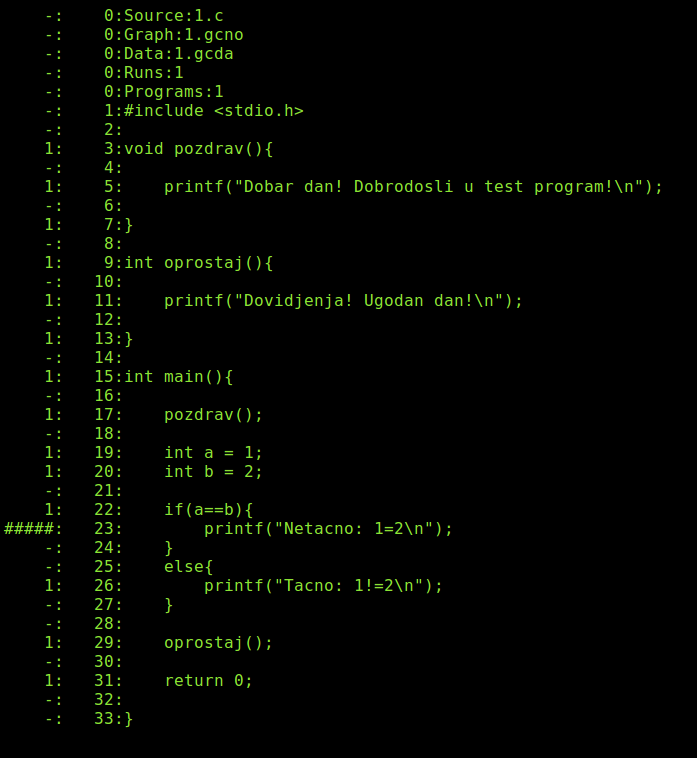
\includegraphics[width=0.5\textwidth]{report.png}
  \caption{osnovni GCOV izveštaj}
\end{figure}


Čitanje podataka iz deljene memorije programa i njihovo skladištenje u gcda fajlove, odvija se kao poslednja instrukcija programa pre kraja izvršavanja (at\_exit). Usled toga, iako analiza GCOV alatom nije striktno vezana za vremenski tok izvršavanja, ne može se vršiti pre kraja programa. Ovo je veliki nedostatak, koji u nekim specifičnim slučajevima može poptuno onemogućiti testiranje pokrivenosti koda. Programi kod kojih je na primer vreme rada izuzetno dugo ili su podaci dostupni i/ili korisni samo tokom rada, kao na primer sistemi za rad u realnom vremenu, serveri ili operativni sistemi, ne mogu koristiti statičku instrumentalizaciju na kraju izvršavanja. Ukoliko imaju ograničene memorijske mogućnosti, što je često slučaj na ovakvim sistemima, ne mogu koristiti ni dinamički pristup programskog prevodioca projekta LLVM. Za obezbeđivanje informacija o pokrivenosti koda ovakvih programa, neophodno je proširiti mogućnosti instrumentalizacije GCC-a na prikupljanje podataka u toku izvršavanja.

Prikaz u vidu pojedinačnih izveštaja za svaki fajl izvornog koda, takođe poseduje određene mane. Svaki izveštaj se nalazi na posebnoj lokaciji u okviru direktorijuma projekta, što otežava njihov pregled kao celine. Dodatne informacije, poput onih o pokrivenosti pojedinačnih funkcija, koje se dobijaju dodavanjem opcija u poziv alata, kao i vrednost pokrivenosti fajla, se ne nalaze u okviru izveštaja, već samo ispisa na standardni izlaz, što uzrokuje potencijalni gubitak tih informacija. Vrednost pokrivenosti koda čitavog projekta se ne izračunava, čime je krajnji rezultat oslabljen za još jednu bitnu informaciju. Potreba za prevazilaženjem ovih mana je uticala na formiranje ideje o novom alatu za vizuelni prikaz GCOV statistike, koji je izgrađen u okviru ovog projekta. 





% ------------------------------------------------------------------------------
\chapter{Zacetak ideje i trnoviti putevi}
\label{chp:ideja}
% ------------------------------------------------------------------------------

\section{Ideja – dinamicki pristup}

\begin{enumerate}
\item Uvod u moj projekat
\item Šta je ovde drukčije i bolje
\item Samo teorija, bez detalja kako tačno radi šta
\end{enumerate}

\section{Razmatrana rešenja}

\begin{enumerate}
\item Dva puta koja su se predamnom bejaše otvorila – da li napadati GCOV alat ili menjati biblioteku
\item Kako i zašto sam odabrala ovo što sam odabrala
\item Lepa pričica da se pokaže da se ipak ulagalo malo mozga u projekat
\end{enumerate}


% ------------------------------------------------------------------------------
\chapter{Implementacija i analiza}
\label{chp:sprovodenje}
% ------------------------------------------------------------------------------

\section{Implementacija}

\begin{enumerate}
\item Biblioteka
\item GUI (signali za prikupljanje podataka, generisanje izvestaja)
\end{enumerate}

\section{Demonstracija i uputstvo za upotrebu}

\begin{enumerate}
\item primer rada biblioteke I GUI-ja sa slikama
\item dobar moment da se naglasi da rad ima primenu na bilo koji kod
\item ne znam jel smem pominjati digitalnu i ko ga sad koristi
\end{enumerate}

\section{Performanse}

\begin{enumerate}
\item da li smo postigli cilj
\item da li možemo isto što i pre, pa i više
\item memorija I bezbednost – test sa Valgrindom
\item složenost – vremenska i prostorna
\item jednostavnost upoterebe
\item ne bi bilo loše ovde pomenuti LLVM i njihovu runtime instrumentalizaciju 
%(LLVM jede memoriju ko lud, jer podatke dampuje u fajlove ali i ugrađuje u samu binariju koja zato naraste mnogo i pravi probleme, dok GCC sve dampuje u fajlove pa je binarija mala).
\end{enumerate}

\section{Primena}

\begin{enumerate}
\item Gde bi sve ovo moglo da radi
\item Ne znam koliko smem odavati na čemu je testirano I na čemu radi
\item Ideja: Ako bi se ovakav jedan alat unapredio I ugradio npr u pejsmejker da signalizira da nešto ne radi kako treba, to što je runtime prikupljanje moglo bi nekome spasiti život
\end{enumerate}


% ------------------------------------------------------------------------------
\chapter{Zaključak}
% ------------------------------------------------------------------------------


\begin{enumerate}
\item Šta je urađeno
\item Koji je značaj toga što je urađeno (gde sad radi – onliko koliko smem da kazem)
\item Šta bi još moglo da se uradi:
\begin{enumerate}
\item Ideja: Ako bi se ovakav jedan alat unapredio I ugradio npr u pejsmejker da signalizira da nešto ne radi kako treba, to što je runtime prikupljanje moglo bi nekome spasiti život
\item Moze mala komparacija sa LLVMom – tipa da se analizira sta je dobro i da se malo unapredi po ugledu na LLVM
\end{enumerate}
\end{enumerate}


% ------------------------------------------------------------------------------
% Literatura
% ------------------------------------------------------------------------------
\literatura

% ==============================================================================
% Završni deo teze i prilozi
\backmatter
% ==============================================================================

% ------------------------------------------------------------------------------
% Biografija kandidata
\begin{biografija}
  \textbf{Marina Nikolić} (\emph{Sombor,
    17. decembar 1992. }) je ... 
\end{biografija}
% ------------------------------------------------------------------------------

\end{document}
